\documentclass[12pt]{article}
%\usepackage[utf8]{inputenc}
%\documentclass[UTF8]{ctexart}
%\usepackage[UTF8, heading = false, scheme = plain]{ctex}
\usepackage{geometry}
%geometry{a4paper,scale=0.9}
\geometry{a4paper,left=1cm,right=1cm,top=1cm,bottom=2cm}
\usepackage{amsfonts}
\usepackage{color}
\usepackage{url}
%\usepackage{biblatex}
\usepackage{amsmath}
\usepackage{amssymb}
\usepackage{latexsym}
\usepackage{cite}
%\addbibresource{ref.bib}
%\bibliography{ref.bib}
\usepackage{caption}
\usepackage{graphicx, subfig}
\usepackage{float}
%\usepackage[fontset=ubuntu]{ctex}
%\usepackage{fontspec}
\usepackage{xeCJK}
%\usepackage[colorlinks,
%anchorcolor=black,
%citecolor=black]{hyperref}
%\setmainfont{SimSun}
\usepackage[section]{placeins}
\usepackage{enumitem}
\usepackage{framed}
\usepackage[framemethod=TikZ]{mdframed}
\usepackage{indentfirst}
\usepackage{setspace}%使用间距宏包
\linespread{1.5}

\title{redis}
\author{leolinuxer}
%\date{June 2020}

\begin{document}
%\setlength{\parindent}{0pt}
\maketitle
\tableofcontents

\section{为什么说Redis是单线程的以及Redis为什么这么快!
\cite{Why_Redis_Is_Single_Threaded_And_Fast}}

\subsection{Redis简介}
Redis是一个开源的内存中的数据结构存储系统,它可以用作:\textbf{数据库、缓存和消息中间件}。

它支持多种类型的数据结构,如字符串(String),散列(Hash),列表(List),集合(Set),有序集合(Sorted Set或者是ZSet)与范围查询,Bitmaps,Hyperloglogs 和地理空间(Geospatial)索引半径查询。\textbf{其中常见的数据结构类型有:String、List、Set、Hash、ZSet这5种}。

Redis 内置了复制(Replication),LUA脚本(Lua scripting), LRU驱动事件(LRU eviction),事务(Transactions) 和不同级别的磁盘持久化(Persistence),并通过 Redis哨兵(Sentinel)和自动分区(Cluster)提供高可用性(High Availability)。

Redis也提供了持久化的选项,这些选项可以让用户将自己的数据保存到磁盘上面进行存储。根据实际情况,可以每隔一定时间将数据集导出到磁盘(快照),或者追加到命令日志中(AOF只追加文件),他会在执行写命令时,将被执行的写命令复制到硬盘里面。您也可以关闭持久化功能,将Redis作为一个高效的网络的缓存数据功能使用。

Redis不使用表,他的数据库不会预定义或者强制去要求用户对Redis存储的不同数据进行关联。

数据库的工作模式按存储方式可分为:硬盘数据库和内存数据库。Redis 将数据储存在内存里面,读写数据的时候都不会受到硬盘 I/O 速度的限制,所以速度极快。

(1)硬盘数据库的工作模式:
\begin{figure}[H]
    \centering
    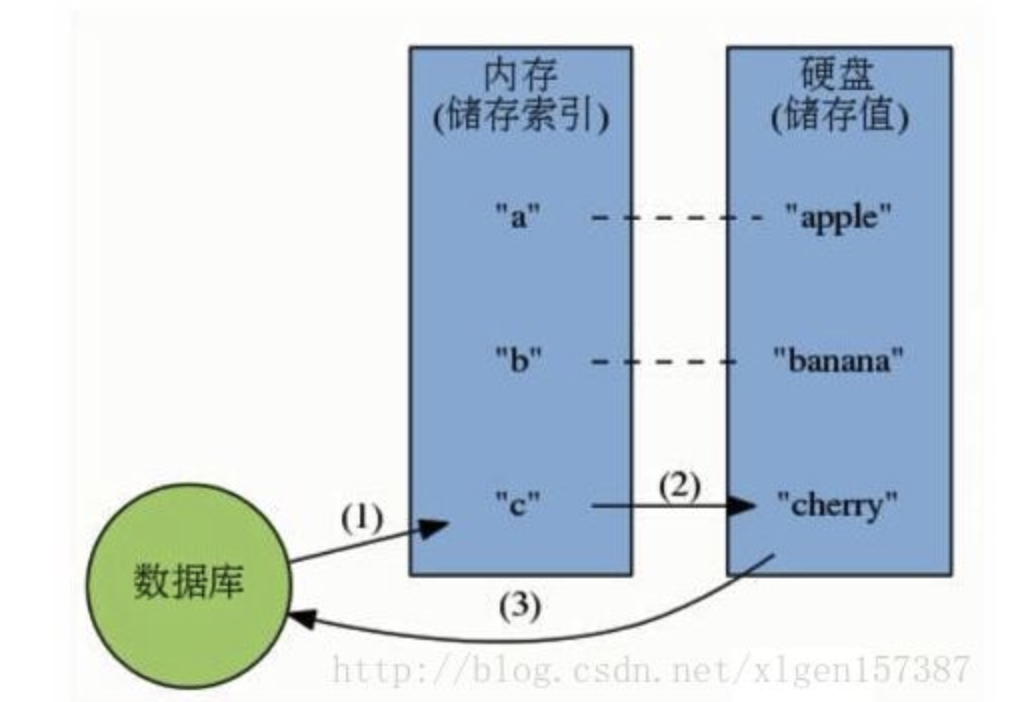
\includegraphics[width=.5\textwidth]{fig/Redis_Fast_1.png}
\end{figure}

(2)内存数据库的工作模式:
\begin{figure}[H]
    \centering
    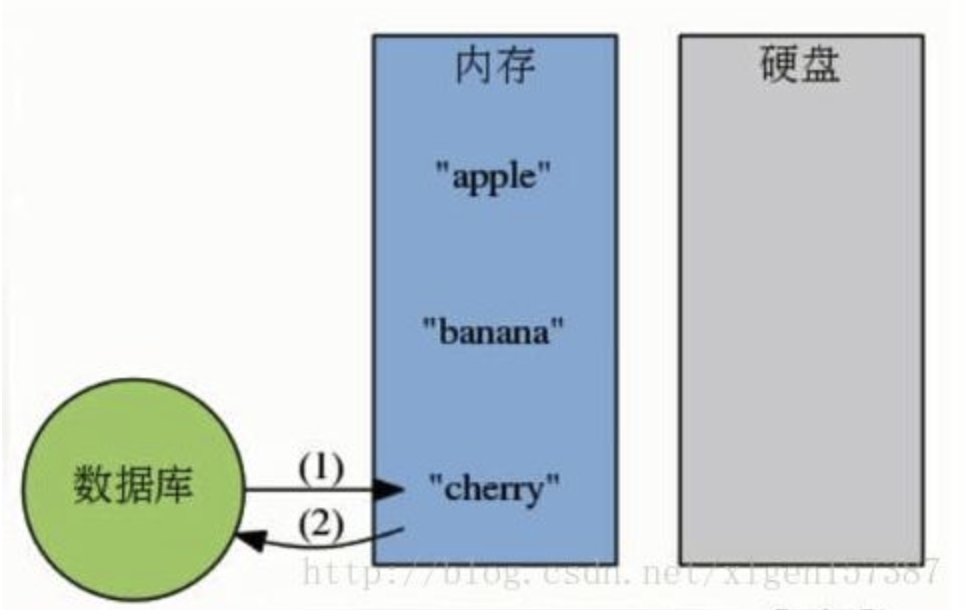
\includegraphics[width=.5\textwidth]{fig/Redis_Fast_2.png}
\end{figure}

看完上述的描述,对于一些常见的Redis相关的面试题,是否有所认识了,例如:什么是Redis、Redis常见的数据结构类型有哪些、Redis是如何进行持久化的等。

\subsection{Redis到底有多快}
Redis采用的是基于内存的采用的是单进程单线程模型的 KV 数据库,由C语言编写,官方提供的数据是可以达到100000+的QPS(每秒内查询次数)。这个数据不比采用单进程多线程的同样基于内存的 KV 数据库 Memcached 差!有兴趣的可以参考官方的基准程序测试《How fast is Redis?》(https://redis.io/topics/benchmarks)
\begin{figure}[H]
    \centering
    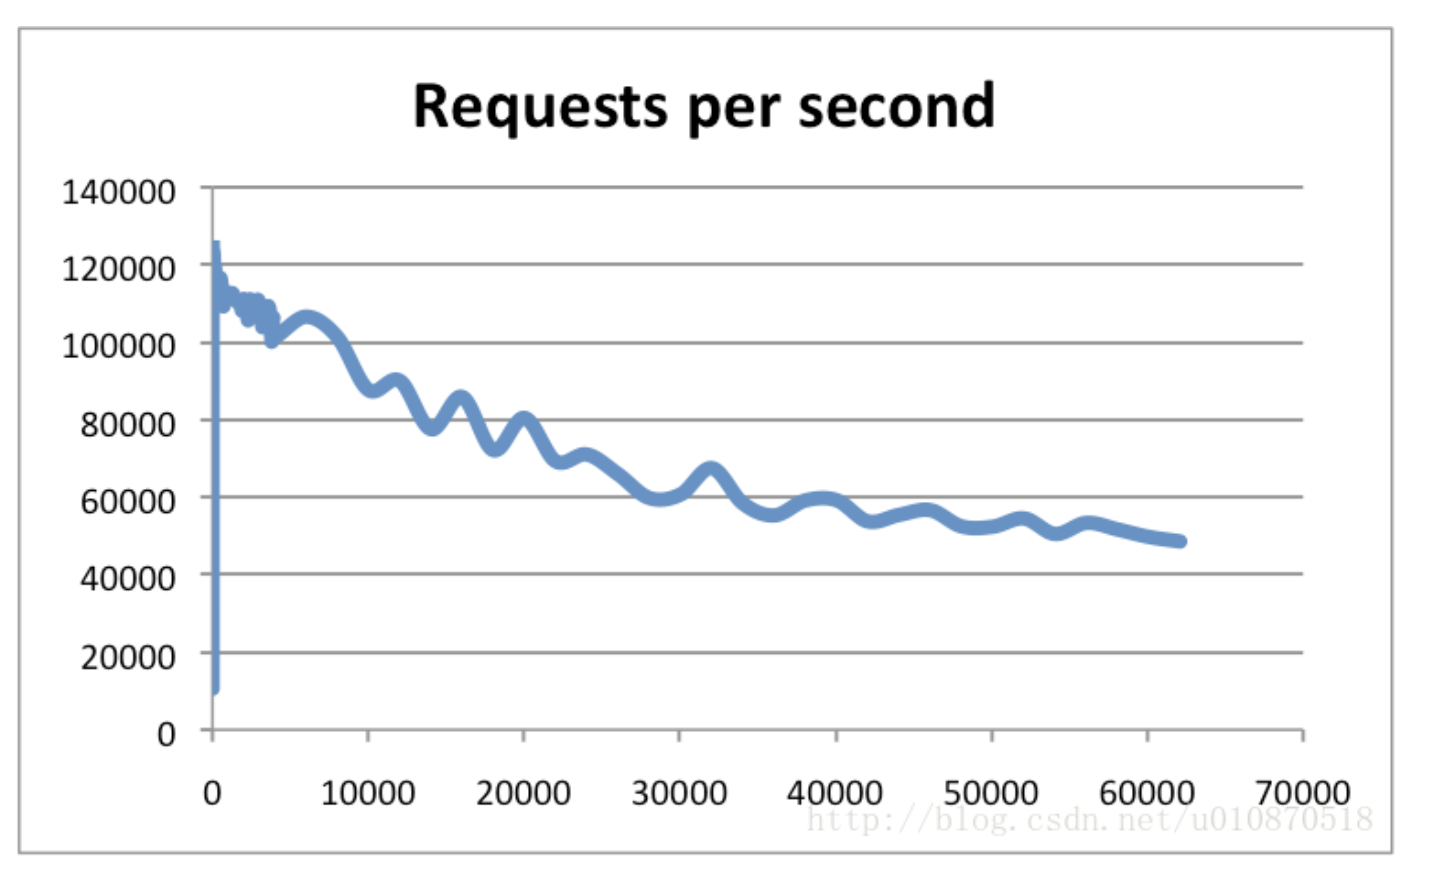
\includegraphics[width=.5\textwidth]{fig/Redis_Fast_3.png}
\end{figure}

横轴是连接数,纵轴是QPS。此时,这张图反映了一个数量级,希望大家在面试的时候可以正确的描述出来,不要问你的时候,你回答的数量级相差甚远!

\subsection{Redis为什么这么快}
1、完全基于内存,绝大部分请求是纯粹的内存操作,非常快速。数据存在内存中,类似于HashMap,HashMap的优势就是查找和操作的时间复杂度都是O(1);

2、数据结构简单,对数据操作也简单,Redis中的数据结构是专门进行设计的;

3、采用单线程,避免了不必要的上下文切换和竞争条件,也不存在多进程或者多线程导致的切换而消耗 CPU,不用去考虑各种锁的问题,不存在加锁释放锁操作,没有因为可能出现死锁而导致的性能消耗;

4、使用多路I/O复用模型,非阻塞IO;

5、使用底层模型不同,它们之间底层实现方式以及与客户端之间通信的应用协议不一样,Redis直接自己构建了VM 机制 ,因为一般的系统调用系统函数的话,会浪费一定的时间去移动和请求;

以上几点都比较好理解,下边我们针对多路 I/O 复用模型进行简单的探讨:

(1)多路 I/O 复用模型

多路I/O复用模型是利用 select、poll、epoll 可以同时监察多个流的 I/O 事件的能力,在空闲的时候,会把当前线程阻塞掉,当有一个或多个流有 I/O 事件时,就从阻塞态中唤醒,于是程序就会轮询一遍所有的流(epoll 是只轮询那些真正发出了事件的流),并且只依次顺序的处理就绪的流,这种做法就避免了大量的无用操作。

\textbf{这里“多路”指的是多个网络连接,“复用”指的是复用同一个线程}。采用多路 I/O 复用技术可以让单个线程高效的处理多个连接请求(尽量减少网络 IO 的时间消耗),且 Redis 在内存中操作数据的速度非常快,也就是说内存内的操作不会成为影响Redis性能的瓶颈,主要由以上几点造就了 Redis 具有很高的吞吐量。

\subsection{那么为什么Redis是单线程的}
我们首先要明白,上边的种种分析,都是为了营造一个Redis很快的氛围!官方FAQ表示,因为Redis是基于内存的操作,CPU不是Redis的瓶颈,Redis的瓶颈最有可能是机器内存的大小或者网络带宽。既然单线程容易实现,而且CPU不会成为瓶颈,那就顺理成章地采用单线程的方案了(毕竟采用多线程会有很多麻烦!)。
\begin{figure}[H]
    \centering
    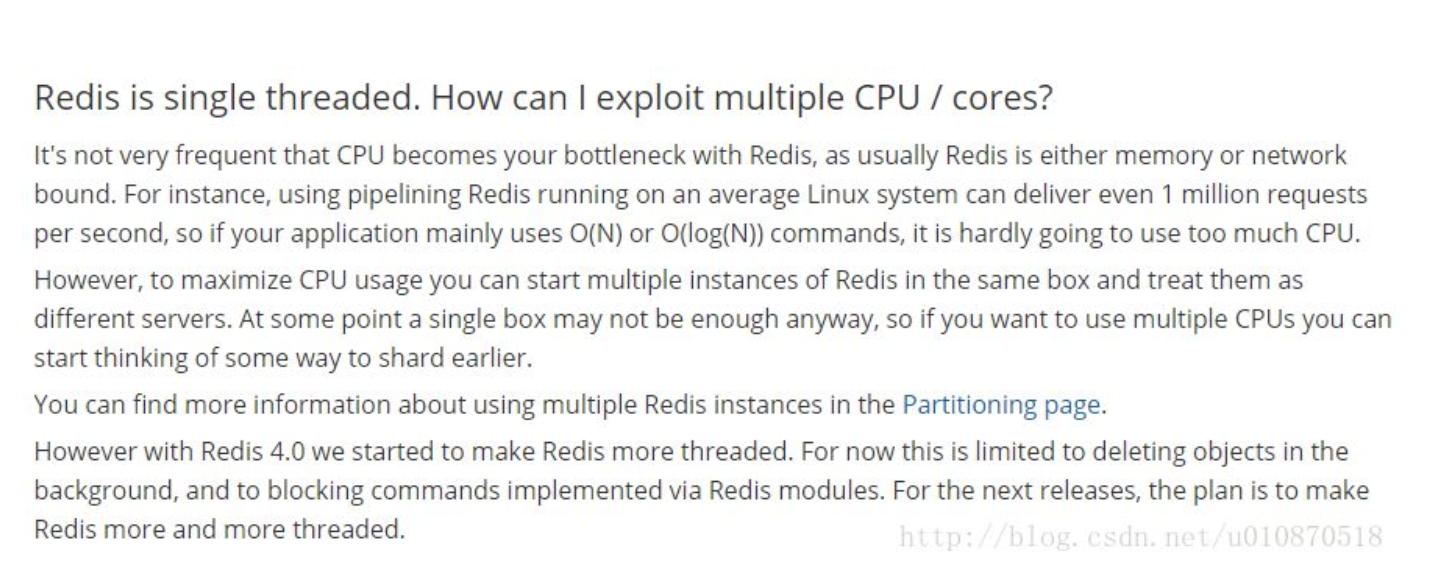
\includegraphics[width=1\textwidth]{fig/Redis_Fast_4.png}
\end{figure}
可以参考:https://redis.io/topics/faq

但是,我们使用单线程的方式是无法发挥多核CPU 性能,不过我们可以通过在单机开多个Redis 实例来完善!

\textbf{警告1}:这里我们一直在强调的单线程,只是在处理我们的网络请求的时候只有一个线程来处理,一个正式的Redis Server运行的时候肯定是不止一个线程的,这里需要大家明确的注意一下!例如Redis进行持久化的时候会以子进程或者子线程的方式执行(具体是子线程还是子进程待读者深入研究);例如我在测试服务器上查看Redis进程,然后找到该进程下的线程:
\begin{figure}[H]
    \centering
    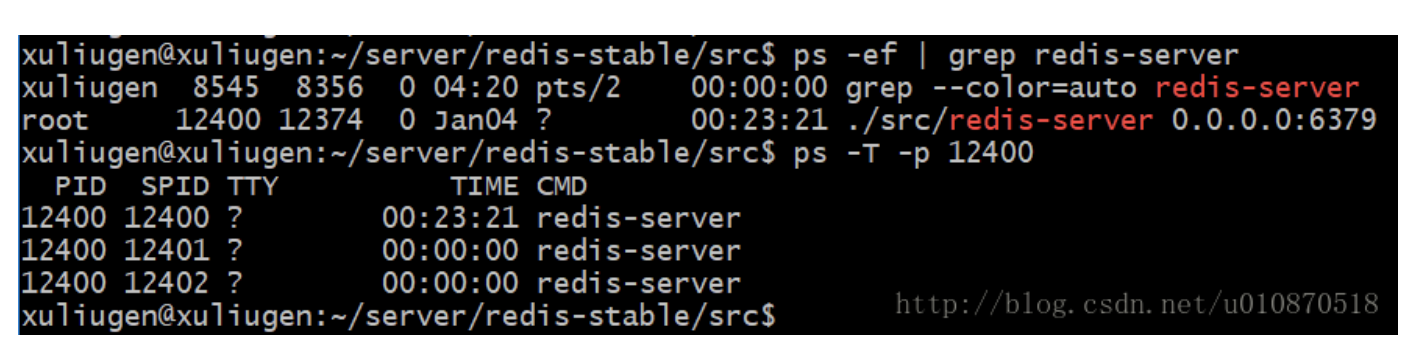
\includegraphics[width=1\textwidth]{fig/Redis_Fast_5.png}
\end{figure}

ps命令的“-T”参数表示显示线程(Show threads, possibly with SPID column.)“SID”栏表示线程ID,而“CMD”栏则显示了线程名称。

\textbf{警告2}:在上图中FAQ中的最后一段,表述了从Redis 4.0版本开始会支持多线程的方式,但是,只是在某一些操作上进行多线程的操作!所以该篇文章在以后的版本中是否还是单线程的方式需要读者考证!

\subsection{注意点}
1、我们知道Redis是用”单线程-多路复用IO模型”来实现高性能的内存数据服务的,这种机制避免了使用锁,但是同时这种机制在进行sunion之类的比较耗时的命令时会使redis的并发下降。因为是单一线程,所以同一时刻只有一个操作在进行,所以,耗时的命令会导致并发的下降,不只是读并发,写并发也会下降。而单一线程也只能用到一个CPU核心,所以可以在同一个多核的服务器中,可以启动多个实例,组成master-master或者master-slave的形式,耗时的读命令可以完全在slave进行。

需要改的redis.conf项:
\begin{figure}[H]
    \centering
    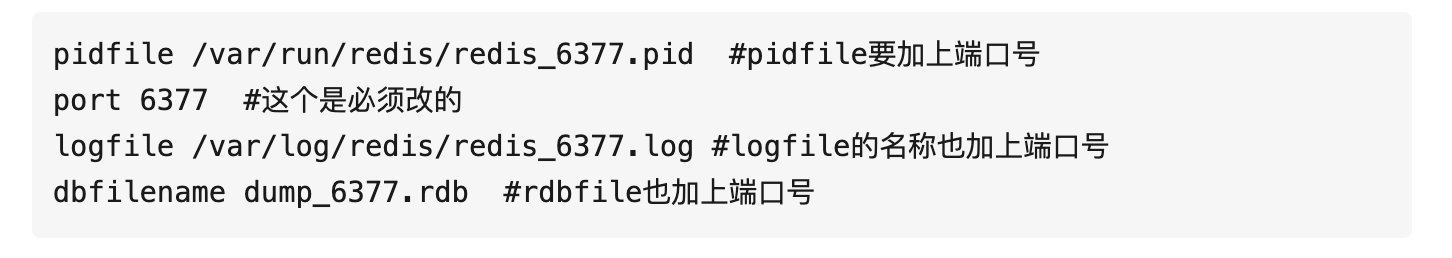
\includegraphics[width=1\textwidth]{fig/Redis_Fast_6.png}
\end{figure}

2、“我们不能任由操作系统负载均衡,因为我们自己更了解自己的程序,所以,我们可以手动地为其分配CPU核,而不会过多地占用CPU,或是让我们关键进程和一堆别的进程挤在一起。”。
CPU 是一个重要的影响因素,由于是单线程模型,Redis 更喜欢大缓存快速 CPU, 而不是多核

在多核 CPU 服务器上面,Redis 的性能还依赖NUMA 配置和处理器绑定位置。最明显的影响是 redis-benchmark 会随机使用CPU内核。为了获得精准的结果,需要使用固定处理器工具(在 Linux 上可以使用 taskset)。最有效的办法是将客户端和服务端分离到两个不同的 CPU 来高校使用三级缓存。

\subsection{扩展}
以下也是你应该知道的几种模型,祝你的面试一臂之力!

1、单进程多线程模型:MySQL、Memcached、Oracle(Windows版本);

2、多进程模型:Oracle(Linux版本);

3、Nginx有两类进程,一类称为Master进程(相当于管理进程),另一类称为Worker进程(实际工作进程)。启动方式有两种:
\begin{itemize}
\setlength{\itemsep}{0pt}
\setlength{\parsep}{0pt}
\setlength{\parskip}{0pt}
    \item 单进程启动:此时系统中仅有一个进程,该进程既充当Master进程的角色,也充当Worker进程的角色。
    \item 多进程启动:此时系统有且仅有一个Master进程,至少有一个Worker进程工作。
    \item Master进程主要进行一些全局性的初始化工作和管理Worker的工作;事件处理是在Worker中进行的。
\end{itemize}
\begin{figure}[H]
    \centering
    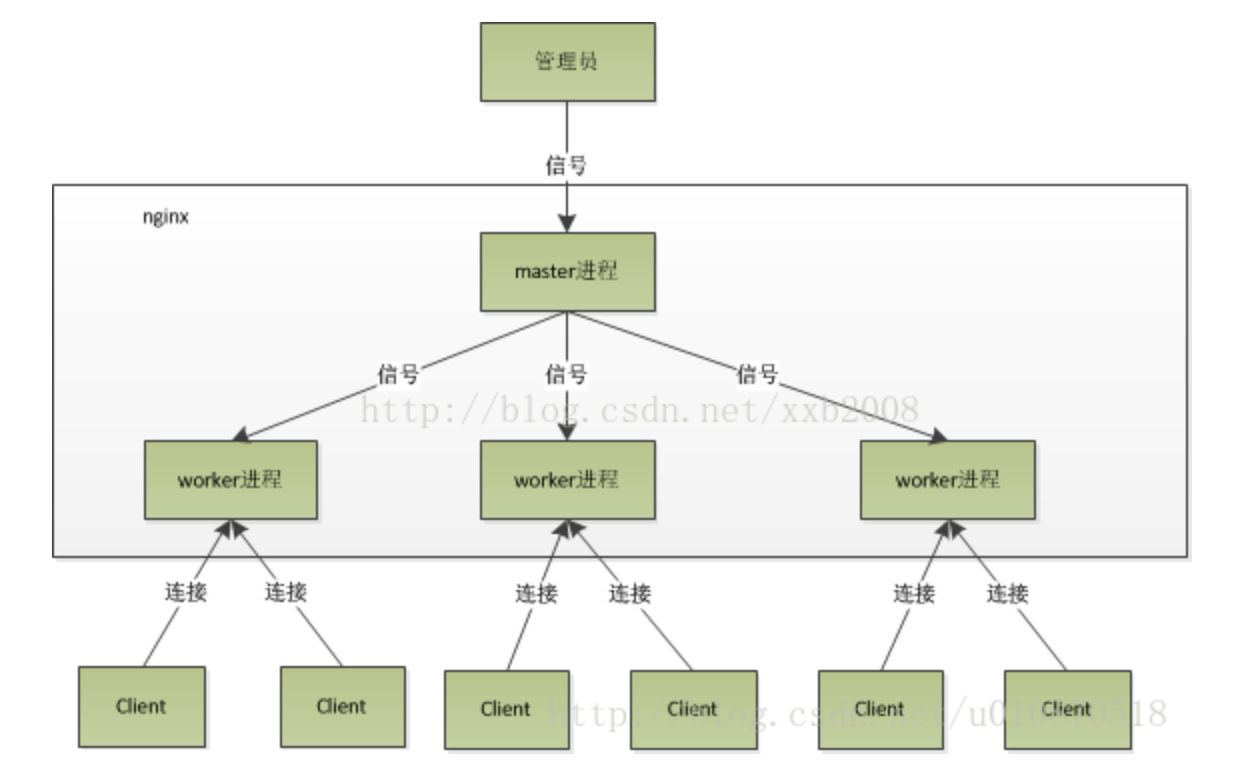
\includegraphics[width=1\textwidth]{fig/Redis_Fast_7.png}
\end{figure}



%\printbibliography
\bibliography{../ref}
\bibliographystyle{IEEEtran}
\end{document}